\section{Proposed Approach}

\begin{figure}[ht!]
    \centering
    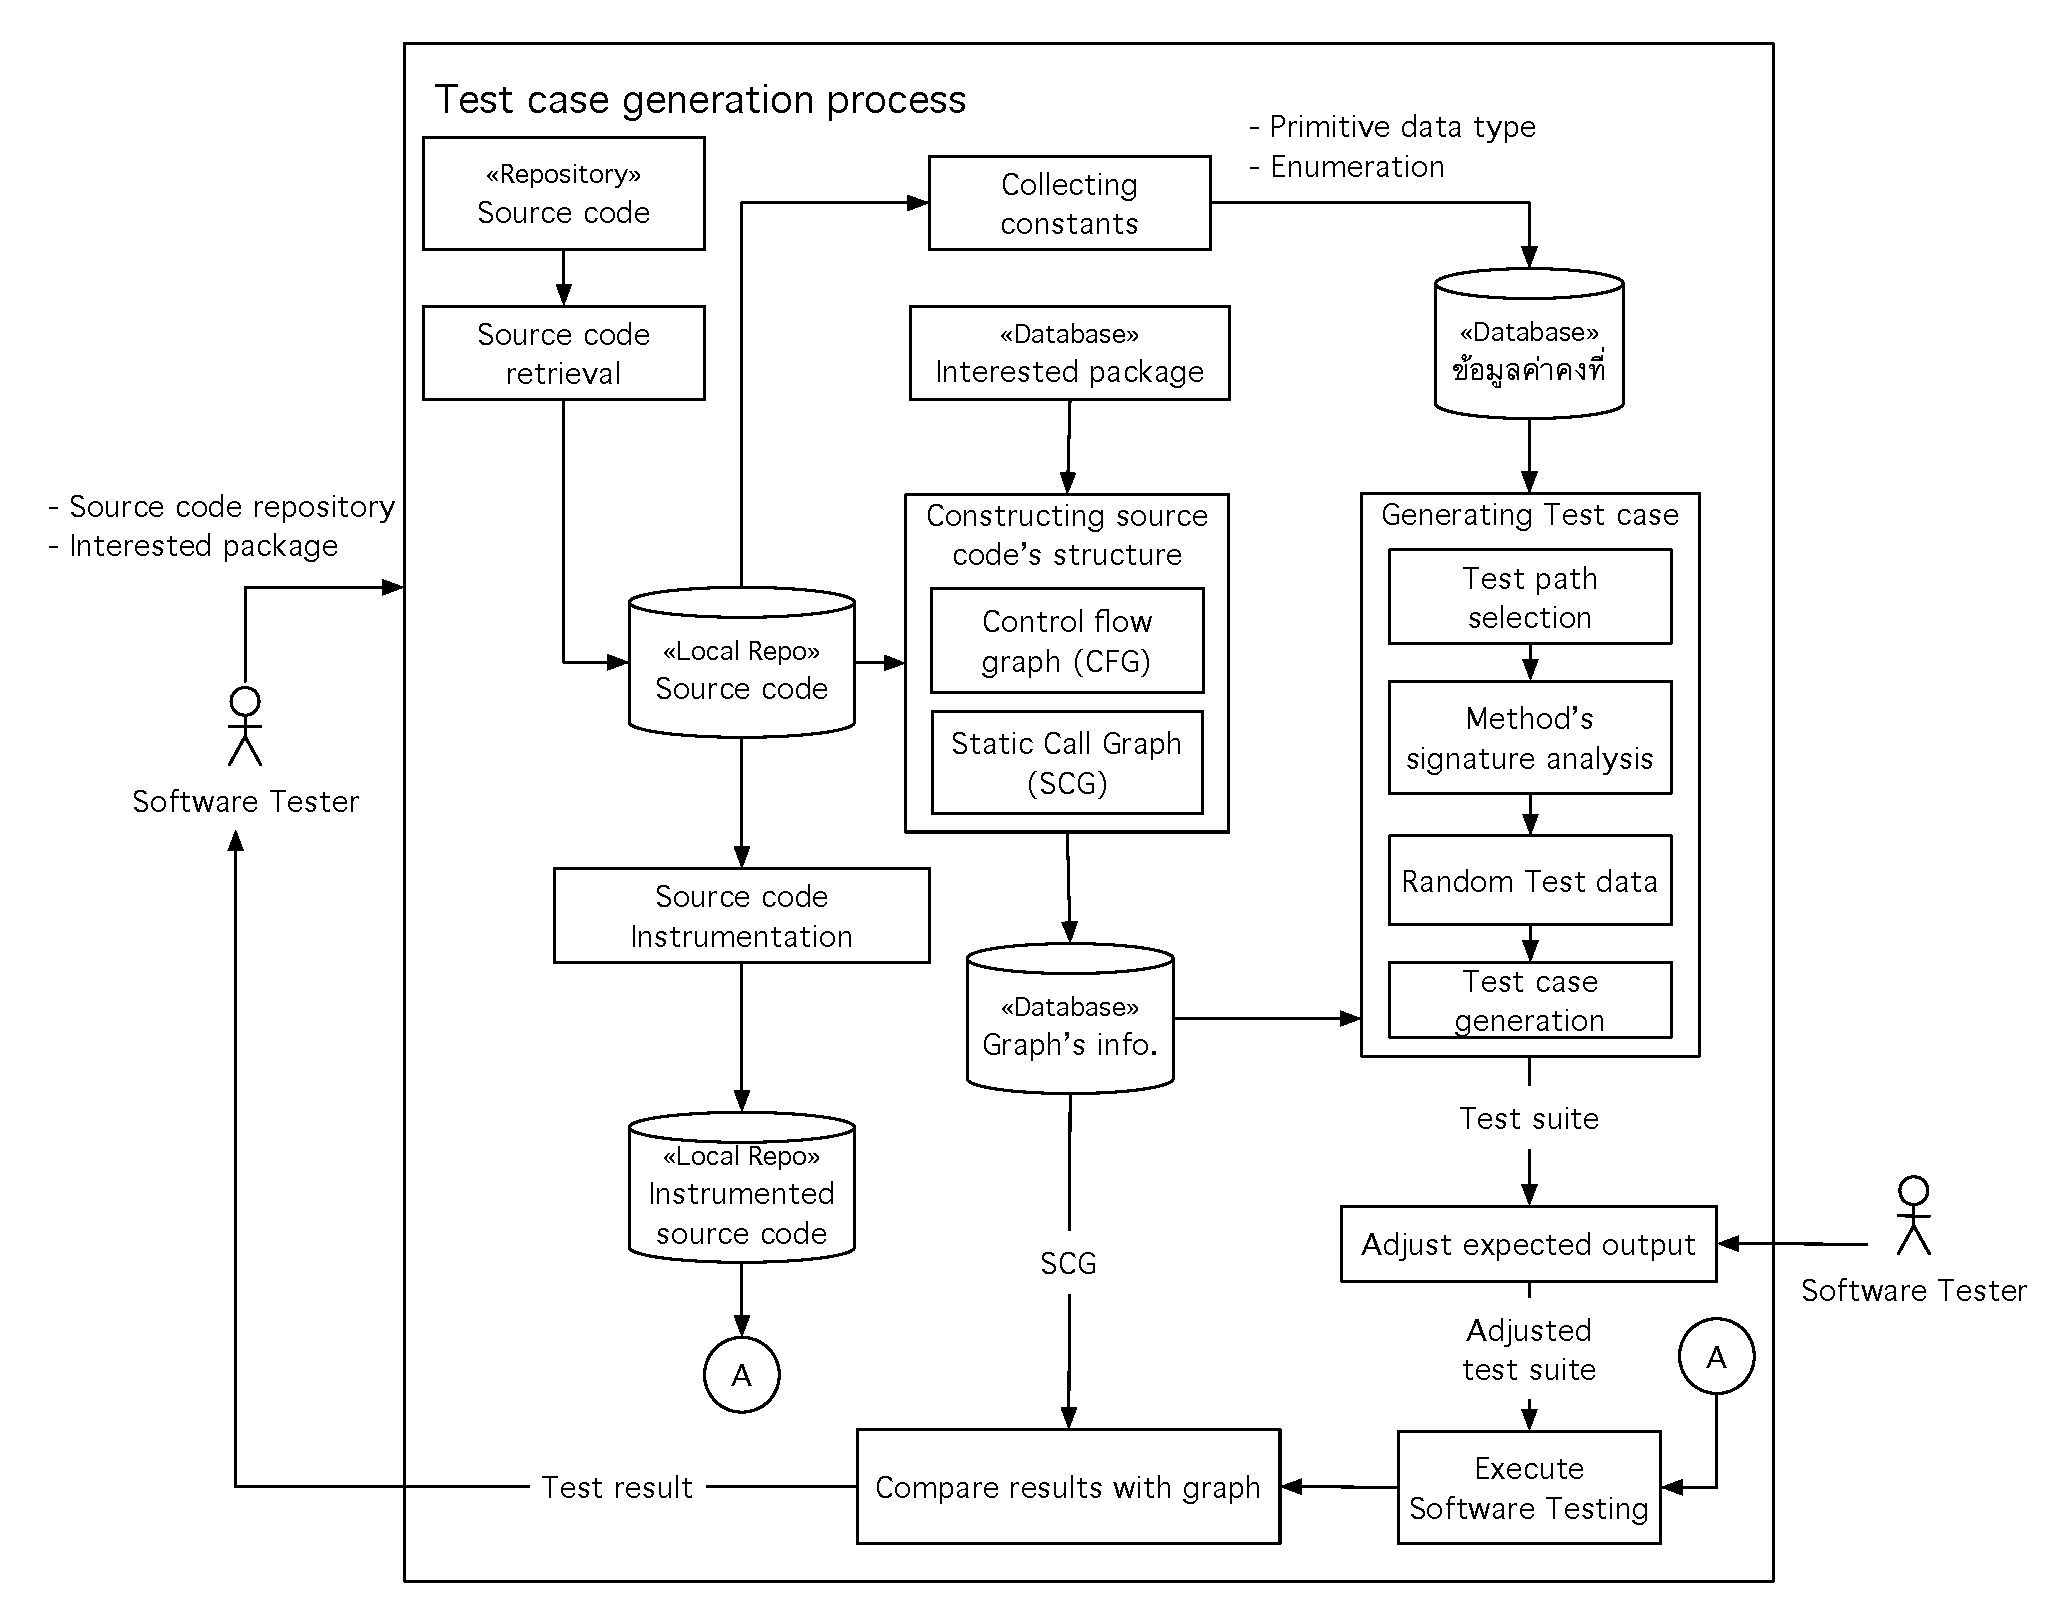
\includegraphics[width=\linewidth]{figures/Methodology}
    \caption{Methodology of Test Case Generation based on Static Data}
    \label{fig:methodology}
\end{figure}

In this section, we present our approach to test case generation 
based on SCG. A set of static data is gathered from source code 
and formed into SCG and CFG. We assure that the generated test case 
conforms to the selected test path. At the last step, we execute 
a test case that comes with instrumentation source code and display 
the result to the software tester. Each step of our approach 
is explained in \figref{fig:methodology}.

\subsection{Source Code Retrieval}

Source code repository is a place to store source code, 
determined by the software tester. At this step, we should 
retrieve source code to access the local repository.

\subsection{Constant Collection}

An object is composed of a primitive data set (booleans, 
numbers, and strings); however, an object which is composed 
of random data will normally fail to satisfy the conditions 
and is not possible to activate a specific path. Therefore, 
we need to find an appropriate value that possibly satisfies 
the criteria. We could say that a predefined primitive value 
in source code can be used to construct an object more potentially 
than the others \cite{McCabe1976}.

This process aims to analyze each class’s files stored within 
a certain package designated by the software tester to collect 
constant values. The collected primitive values should 
also lead to random satisfying values in order to cover 
the test paths \cite{McCabe1976}.

\subsection{Constructing Source Code’s Structure}

In order to form a satisfying condition for source code, 
the software tester has to understand its structure. Therefore, 
this process is to create graphs, CFG and SCG, which represent 
the structure of source code and eliminate infeasible paths. 
When the process ends, source code structure, the graphs, 
and all possible paths will be stored in the database. 
Soon after, the generated test case will retrieve data 
from the database to generate another test case that conforms 
to the selected test paths. For more detail, each step 
is clearly discussed as follows:

\subsubsection{Control Flow Graph Construction}

Source code within the assigned package is retrieved from 
the repository given by a software tester, and parses each statement 
into nodes is assigned. Then, it will assign a relationship 
of the source node and the other nodes, which work after 
the previous node, until nodes are all connected. Finally, we must 
keep all the feasible paths and source node to sync all of them in 
the form of graph in the database. For example, if $C_1$, $C_2$, 
and $C_3$ are classes within the interested package which contains 
method sets: \{$m_{11}$, $m_{12}$\}, \{$m_{21}$, $m_{22}$, $m_{23}$\}, 
and \{$m_{31}$, $m_{32}$\} respectively, CFG will be created 
from each method in a certain class.

From this process, we create CFG from source code to represent 
the source code structure. Furthermore, we also gather data 
from the steps of creating an object. These steps should be used 
as a reference in the test case generation process.

\subsubsection{Static Call Graph Construction}

This process collects the static data from source code 
for SCG construction. To perform this process, source code 
should be retrieved from the local repository. Then, calling statements 
that call to another class should be collected. A method that 
contains calling statements should be assigned to calling method, 
and a method is called in calling statement should be assigned 
to called method. To create SCG, in which each node represents classes 
in SUT and each edge represents the relationship between nodes. 
At the final phase, each edge will be labeled by the calling and 
called methods as shown in \figref{fig:relationship}

\begin{figure}[bh!]
\centering
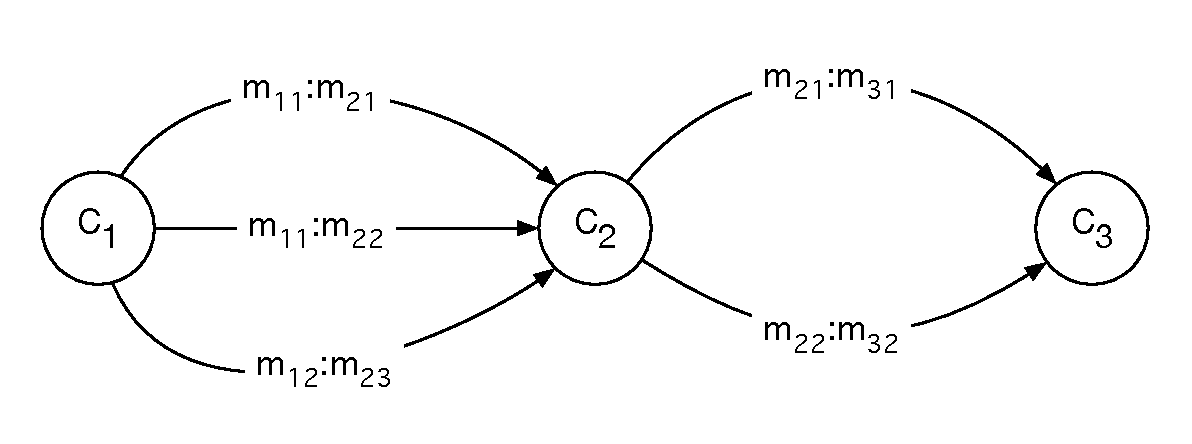
\includegraphics[width=\linewidth]{figures/Relationship-between-Classes}
\caption{Relationship between Classes $C_1$, $C_2$ and $C_3$}
\label{fig:relationship}
\end{figure}

\subsection{Source code instrumentation}

This process adds instrumentation message that displays 
a specific message when the test case has exercised through 
the lines. To make sure that the generated test cases have 
already covered all SCG’s branches (Branch coverage), at least once. 
Source code should be instrumented for monitoring if all branches 
are covered.

\subsubsection{Method Entry and Existence}
In statement instrumentation, the instrumentation message is 
added right after method declaration statement and before method 
ending or returning values. Message from this statement shows 
that test cases are able to exercise through methods 
between classes on test paths.

\subsubsection{Predicate Execution}
Selected test paths can be consisted of several predicate nodes. 
For this statement type, instrumentation message 
is added right after predicate statements.

\subsubsection{Calling Method}
Displaying message while methods between classed are invoked 
is the main goal of this approach. Instrumentation message 
is added right before and after finding these statements 
in order to display the message before and after invoking 
for method, respectively. For the message analysis, we analyze 
message from the entry method and explain the execution path 
for both invoking and invoke method.

After this process, instrumentation source code 
will be archived in the local repository.

\subsection{Test Case Generation}

In our approach, test cases are generated based on 
static data collected from source code. Previously, the constant 
and source code structures collected. This process analyze the data 
and generates test data and test cases in order to exercise 
each SCG’s branch at least one time. The process 
is shown as in \figref{fig:activitiesTC}

\subsubsection{Test Path Selection}
This process starts with retrieving all test paths of SCG and CFG 
structure formed in the database. Then, we should consider 
each pair of the SCG nodes. After that, the calling and called methods 
should be extracted from each edge label, one by one. For the next step, 
we should select CFG for calling node in order to analyze 
the test paths by finding the shortest path that contains calling nodes 
which represent to calling statements. This means that the first node pair 
of the test path is being selected. Next, the previous tail node 
is set to be the head node. Calling method is set to previously 
called method. Then, we repeat the test path selection steps in order to 
find all of the test paths. This is to achieve the branch coverage.

From SCG of class $C_1$, $C_2$, and $C_3$ as shown in \figref{fig:relationship}, 
we can get started from the nodes of $C_1$ and $C_2$ ($C_1$ is the head node, 
while $C_2$ is the tail node). After that, we have to extract the name of 
the calling and called methods from each of the edge labels. 
Therefore, $m_{11}$ and $m_{21}$ retrieved from the above edge should be 
calling and called methods respectively. After that, we have to find 
calling statements and called method, which are $m_{21}$, in $m_{11}$ from 
the structure of m11 as shown in \figref{fig:cfgOfMethod}, given that node 16 is invoking node 
(invoking statement). Now, we have already generated test paths, $11-12-14-16-18-19$, 
from m11 to cover all the branches ($C_1$, $C_2$, $m11:m12$). Then, the head node 
will be changed from $C_1$ to $C_2$, and the invoking method will be changed 
from $m_{11}$ to $m_{21}$. When it comes to this final step, we need to repeat all 
over again if there are any edge labels that start with the invoking method. 
If there are no any edge labels with the invoking method left, we have to set 
the invoking method on another invoking method that is left on 
the previous head node.

\begin{figure}[ht!]
\centering
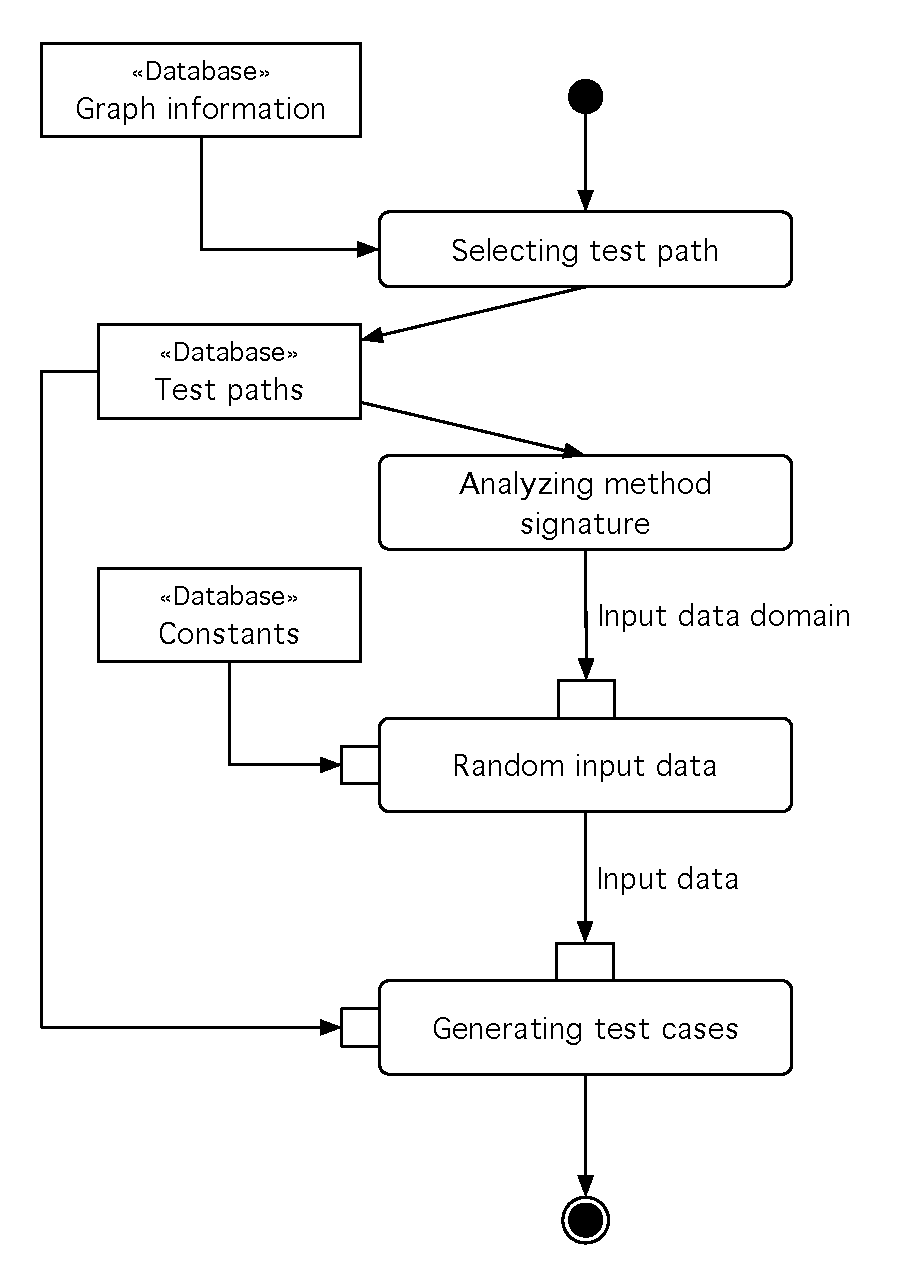
\includegraphics[width=0.7\linewidth]{figures/Activities}
\caption{Activities in Test Caset Generation Process}
\label{fig:activitiesTC}
\end{figure}

\begin{figure}[hb!]
\centering
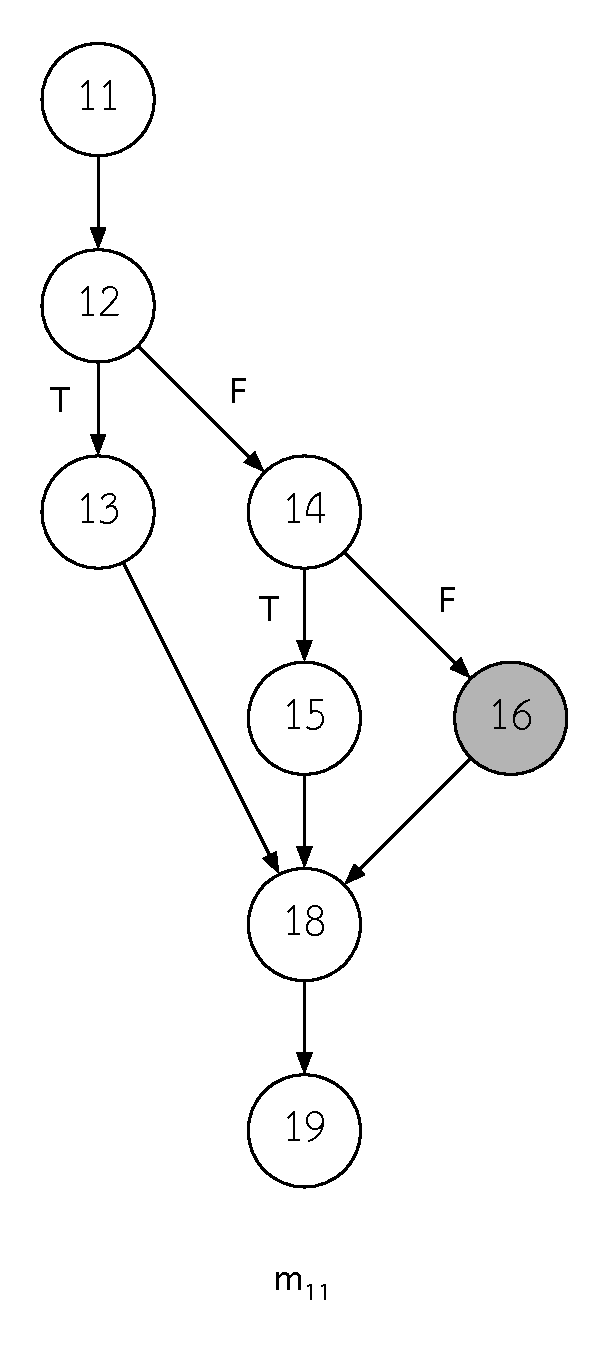
\includegraphics[width=0.4\linewidth]{figures/CFG-of-m11-in-c1}
\caption{Control Flow Graph of method $m_{11}$ of class $C_1$}
\label{fig:cfgOfMethod}
\end{figure}

According to the steps explained above, the test cases can be generated 
as shown in \tabref{tab:generatedTestCase}

\begin{table}[!t]
\renewcommand{\arraystretch}{1.3}
\caption{Generated Test Case from a Static Call Graph}
\label{tab:generatedTestCase}
\centering
\begin{tabular}{cl}
\hline
ID & Test Path \\ \hline
1  & ($C_1$, $C_2$, $m_{11}:m_{21}$) - ($C_2$, $C_3$, $m_{21}:m_{31}$) \\ \hline
2  & ($C_1$, $C_2$, $m_{11}:m_{22}$) - ($C_2$, $C_3$, $m_{22}:m_{32}$) \\ \hline
3  & ($C_1$, $C_2$, $m_{12}:m_{23}$) \\ \hline
\hline
\end{tabular}
\end{table}

For the test paths retrieved from SCG in \tabref{tab:generatedTestCase} we have to consider CFG 
of method $m_{11}$ within class $C_1$, method $m_{21}$ within class $C_2$, and finally 
method $m_{31}$ within class $C_3$. CFG shown in \figref{fig:callingStatement} is the CFG 
of $m_{11}$, $m_{21}$ and $m_{31}$ respectively. The generated test paths should be tuple of 
(($11$, $12$, $14$, $16$)$m_{11}$, ($10$, $11$, $17$)$m_{21}$, 
($10$, $11$, $12$, $14$, $18$, $19$)$m_{31}$, ($17$, $18$, $19$)$m_{21}$, ($16$, $18$, $19$)$m_{11}$). 
Finally, all test paths are sent to the signature analysis method for the next process.

\begin{figure}[ht!]
\centering
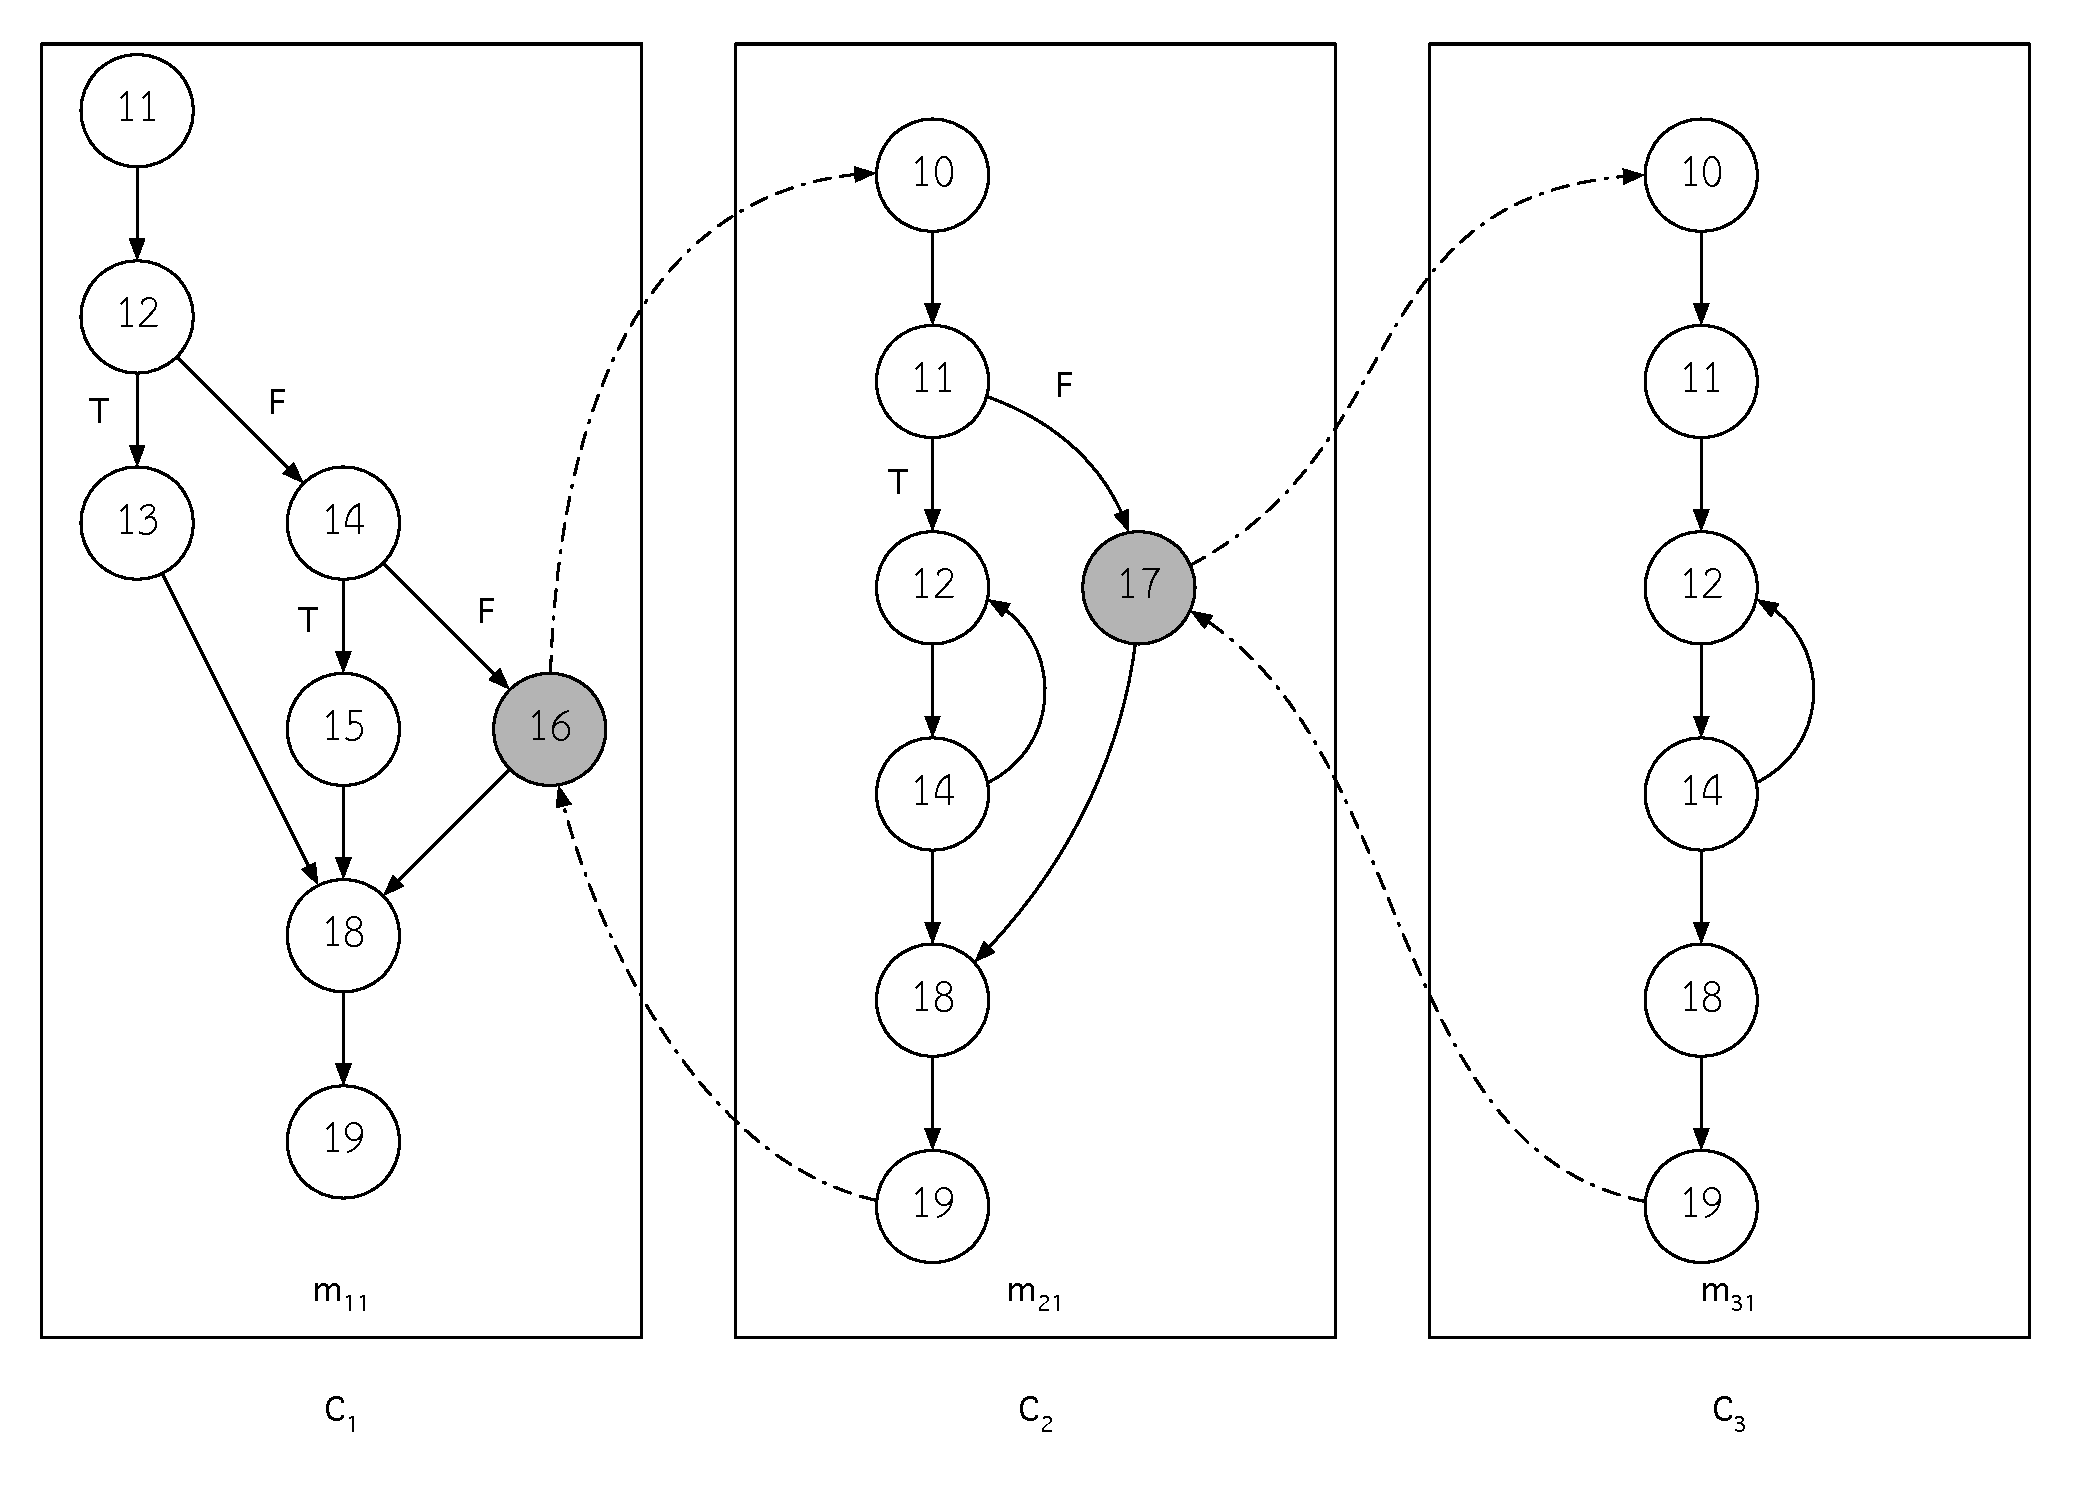
\includegraphics[width=\linewidth]{figures/Calling-statements-of-Classes}
\caption{Calling Statement between Method $m_{11}$ of $C_1$, Method $m_{11}$ of Class $C_2$, and Method $m_{31}$ of Class $C_3$}
\label{fig:callingStatement}
\end{figure}

\subsubsection{Signature Analysis Methods}
This process is performed in order to guide an input domain for random input process 
by signature analysis method, calling and called methods and test path that are transferred 
from the previous process, including the predicate nodes that are found on the test path \cite{Ma2016}. 
For example, a selected path (\figref{fig:callingStatement}) has 3 predicate nodes i.e. 
node $12$, node $14$ of method $m_{11}$, and node $11$ of method $m_{21}$. The random input data 
are guided by conditions found in predicate node.  Thus, input data should conform 
to each predicate node and each predication node must be in line with the conditions provided in 
\figref{fig:conditionsPredicate}

\begin{figure}[ht!]
    \centering
    \makebox[0.7\linewidth][l]{$m_{11}:12~studentScore~>~80$} \par
    \makebox[0.7\linewidth][l]{$m_{11}:14~studentScore~>~50$} \par
    \makebox[0.7\linewidth][l]{$m_{21}:11~true~>~hasQuizScore$}
    \caption{Conditions in Predicate Nodes}
    \label{fig:conditionsPredicate}
\end{figure}
\begin{figure}[ht!]
    \centering
    \makebox[\linewidth][l]{$m_{11}(String\,studentID,\,float\,studentScore)\,:\,String$} \par
    \makebox[\linewidth][l]{$m_{21}(String\,studentID)\,:\,float$} \par
    \makebox[\linewidth][l]{$m_{31}(String\,studentID)\,:\,float$}
    \caption{Method Signatures of $m_{11}$, $m_{21}$, and $m_{31}$}
    \label{fig:methodSignature}
\end{figure}

This is where the test data generation has considered each predicate node provided above. 
Test data should be generated to conform with predicated found in node $m_{11}:12$, 
$m_{11}:14$ and $m_{21}:11$ in order to activate the test case.

With the signature method $m_{11}$, $m_{21}$ and $m_{31}$ as given in \figref{fig:methodSignature}, 
when the test data has considered each predicate above, it is to say that, there is only $studentScore$ 
that we have to consider and ignore for $hasQuizScore$. Because $hasQuizScore$ does not exists in 
method signature. Finally, studentScore should conform predicate node must be lower than 
or equal to $80$ and $50$.


\subsubsection{Random Input Data}
Previously, random data has already randomized the value, but the method could have been more 
than one parameter. That is, each parameter of the method has to be considered. For the parameter 
found in the predicate nodes, it already has a guiding value from the previous process. 
On the other hand, parameters that are not found in the predicate nodes must be randomized 
by using constant value gathered from the constant collection process \cite{Ma2016}

\subsubsection{Test Case Generation}
For this process, test path should be converted to a set of test cases. Test case generation 
must conform to the steps of object creation that can be found in the test path, 
including of the test data formed in the previous process.

\subsection{Expected Output Adjustment}
At this process, test cases are generated; however, they are not actually executed, 
because our approach has gathered only the static data and regardless the behavior method 
such as methods of returning values or input values that do not appear on the test paths. 
The software tester must adjust these values to satisfy the test paths, altogether 
with considering the behavior method.

\subsection{Software Testing Execution}
After expected output adjusted, the software tester has achieved to adjust expected outputs 
of the test cases, the test case must be executed with the instrumented source code 
retrieved from the source code instrumentation process in the local repository. During 
the execution process of the test, we should collect instrumentation messages 
that are displayed when the test cases traverse through nodes of test path.

\subsection{Result Comparison to Graph}
In order to verify a generated test case, we should create a traversing path from 
the instrumentation message that is collected from the previous process and display 
the execution result to the software tester.
